\section{Implementation}\label{sec:impl}
%%%%%%%%%%%%%%%%%%%%%%%%%%%%%%%%%%%%%%%%%%%%%%%%%%%%%%%%%%%%%%%%%%%%%%%%%%%%%%%%%%%%%%%%%%%%%%%%%%%%%%%%%%%%%%%%%%%%%%%

\module{From in-place to out-of-place writes.}
To evaluate our techniques, we extend LeanStore~\cite{DBLP:journals/pvldb/Leis24}, a B-tree system that originally performs in-place writes.
We integrate vmcache~\cite{DBLP:journals/pacmmod/LeisA0L023} as the buffer pool to support 1:N PID-offset mappings, 
enabling out-of-place writes.
The resulting prototype, \emph{Z (Zoned) LeanStore}, shows that our optimizations apply to an arbitrary page-based system.
\revision[R2.W1]{We first outline the write path to illustrate how the optimizations work together.
We then describe necessary extensions to other components~\cite{WObtree, WiredTiger_Checkpoint_Arch} to implement our techniques without compromising durability. }


\subsection{Design Overview}

\module{How the main components support optimizations.}
We modify four DBMS components: the buffer manager, I/O interface, space manager, and garbage collector.
The buffer manager computes each page’s EDT using write timestamps stored in the page header.
The I/O interface performs compression, page packing, and selects the backend based on the SSD type (e.g., ZNS or FDP).
Storage space is partitioned into zones, sized according to the inferred SSD GC unit.
The space manager maintains PID-offset and reverse mappings, tracks zone metadata, and selects zones for placement based on GDT.
The GC reclaims space in both foreground and background, choosing victims based on GDT while preserving the NoWA pattern.

\begin{figure}[t]
    \centering
          \setlength{\abovecaptionskip}{3pt} % space above caption
  \setlength{\belowcaptionskip}{0pt} % space below caption (usually inside float)
    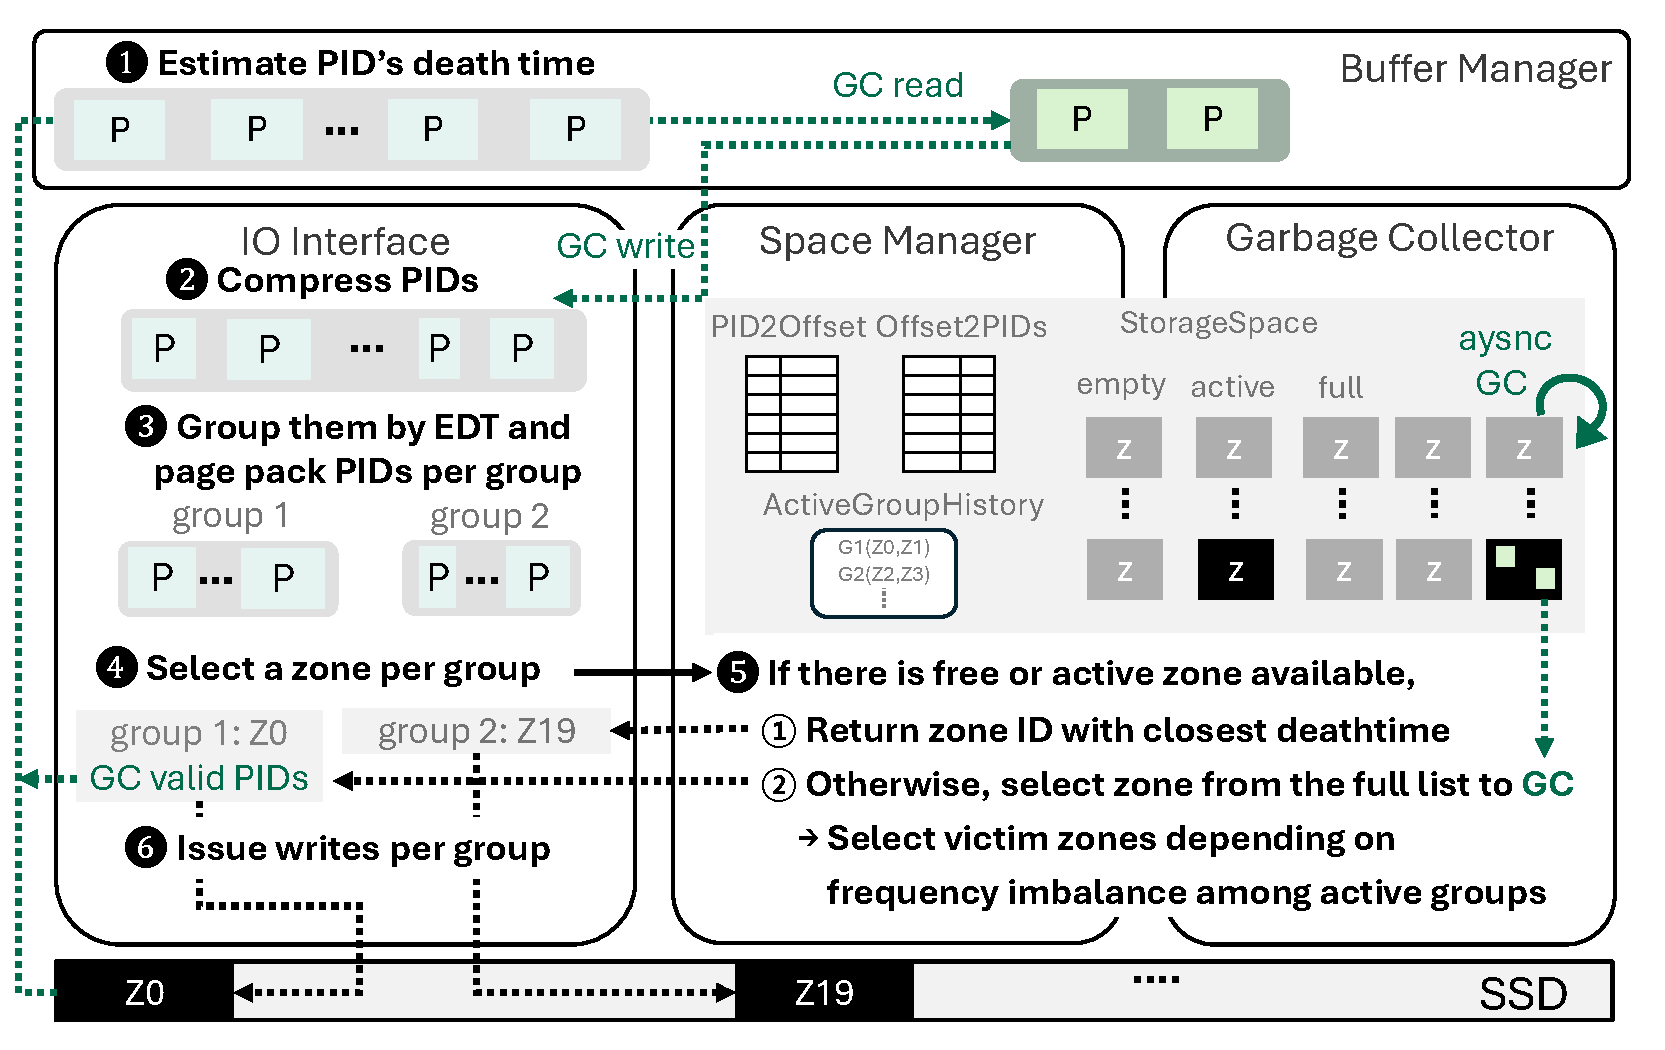
\includegraphics[clip, width=0.5\textwidth]{figures/writepath.pdf}
    \caption{Overview of the write path with all optimizations.}
    \label{fig:writepath}
\end{figure}

\module{Write path.}
Write requests follow the path illustrated in \cref{fig:writepath}.
Suppose a batch of PIDs must be flushed upon eviction.
First, each PID’s EDT is computed from previous write LSNs stored in the page header.
The PID, its contents, and its EDT are passed to the I/O interface (\ding{182}), which compresses pages (\ding{183}) and groups PIDs with similar EDTs (\ding{184}).
The space manager then assigns a target zone for each group (\ding{185}): 
if active zones exist, the one whose average EDT is closest is chosen (\textcircled{1}); 
otherwise, a new zone is opened from the empty or full list, respecting the active-zone limit.
If a zone is full, GC is triggered (\textcircled{2}).
During GC, valid pages not in the buffer pool are read in and rewritten following the same write path (\ding{182}-\ding{184}).
When multiple zones are reclaimed, valid PIDs are sorted by descending EDT and written into zones with the highest invalidation counts, placing the coldest pages into the coldest zones.
After GC completes, the originally requested write proceeds (\ding{187}).

%%%%%%%%%%%%%%%%%%%%%%%%%%%%%%%%%%%%%%%%%%%%%%%%%%%%%%%%%%%%%%%%%%%%%%%%%%%%%%%%%%%%%%%%%%%%%%%%%%%%%%%%%%%%%%%%%%%%%%%


\subsection{Implementation Details}

\module{Sharing the buffer pool as a cache for GC.}
The GC shares the buffer pool with worker threads to perform GC I/Os, avoiding memory partitioning and allowing full utilization when GC is inactive.
This reduces disk reads during GC as some valid PIDs may already be in memory.
Although GC may harm the hit ratio, it often acts as a prefetcher, as GDT-based GC tends to load PIDs that will be accessed soon, thus reducing its negative impact.

\module{Securing clean buffer frames for GC reads.}
A full buffer pool can create contention between eviction and GC, as both require free frames.
To avoid eviction writes during GC, only clean frames may be reused for GC reads.
Thus, the system maintains a minimum reserve of clean pages, integrated with fuzzy checkpointing~\cite{leanstore-logging}.
If the reserve falls below the threshold, the checkpointer flushes additional pages during non-GC phases.
In practice, this mechanism is rarely invoked because regular checkpointing already keeps enough clean frames available.

\module{I/O buffer for compression and page packing.}
The I/O interface uses a per-thread temporary buffer to issue I/O requests.
PIDs are compressed with LZ4~\cite{compression/lz4}, grouped by GDT, page-packed, and issued as a single I/O request.
For reads, a 4~KiB-aligned buffer fetches the compressed data; after decompression, only the requested PID is inserted into the buffer pool.

\module{Space metadata.}
The space manager maintains three types of metadata and updates them whenever a write occurs.
First, \texttt{PID2OffsetTable} maps each PID to its on-disk offset and compressed size.
Second, \texttt{StorageSpace} provides the reverse mapping.
It tracks which PIDs occupy each 4~KiB offset and stores zone metadata such as fill factor, page and zone invalidation counts, average EDT, and state.
Finally, to implement the NoWA pattern, \texttt{ActiveGroupHistory} records the active group each time a new set of zones is opened.

\module{Supporting various GC strategies.}
The garbage collector activates whenever active zones nearly run out of device space.
Depending on the enabled configuration, it runs victim selection strategies such as greedy, GDT-based GC, and/or NoWA-aware GC.
This way, the user can run GC that fits the workload characteristics.

\revision[R2.W2]{
\module{Compatibility with ZNS SSDs and FDP.}
The I/O layer detects the device type and selects the appropriate backend via \texttt{ioctl}.
Standard SSDs use an \texttt{io\_uring}-based backend.
For ZNS SSDs, writes use zone-append operations, zones are reset after GC, and the system tracks the device’s limit on open zones.
For FDP-enabled SSDs, we query the RU size and number of RU handles, set the maximum number of active zones accordingly, and apply placement hints by mapping zone IDs modulo the number of handles.
}

\revision[R2.W1, R2.D1]{
\module{Logging and recovery.}
We use per-thread logs with continuous checkpointing~\cite{leanstore-logging}.
To ensure recoverability, the system logs \texttt{PID2Offset} updates.
We enforce standard write-ahead rules: page data is persisted before its mapping update is committed.
Each checkpoint persists snapshots of the \texttt{PID2OffsetTable} and the \texttt{ActiveGroupHistory}.
Recovery is performed by first locating the checkpoint LSN, reloading these snapshots, and replaying subsequent WAL entries; this naturally also reconstructs metadata.
Finally, the \texttt{StorageSpace} layout is rebuilt from the final \texttt{PID2Offset-} \texttt{Table}.
}


\begin{figure*}[t]
    \centering
      \setlength{\abovecaptionskip}{3pt} % space above caption
  \setlength{\belowcaptionskip}{0pt} % space below caption (usually inside float)
    \begin{subfigure}{0.23\textwidth}
        \centering
        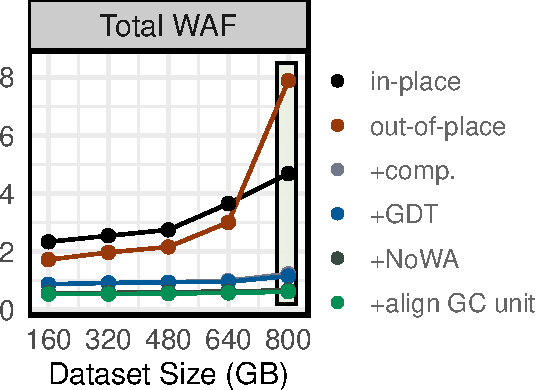
\includegraphics[width=\linewidth]{figures/drilldown.pdf}
        \caption{Total WAF}
        \label{fig:drilldown:a}
    \end{subfigure}
    \hfill
    \begin{subfigure}{0.34\textwidth}
        \centering
        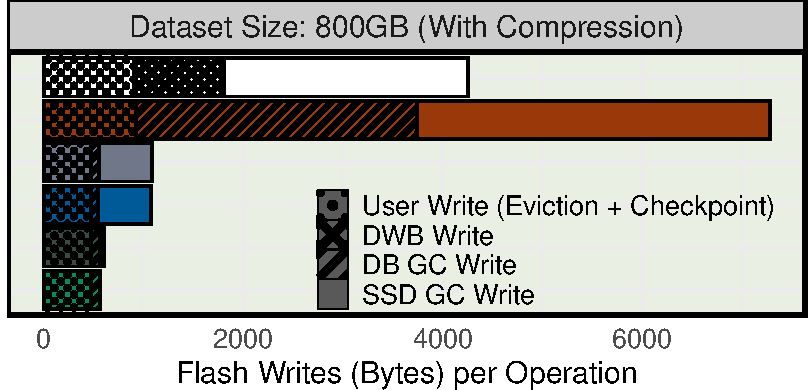
\includegraphics[width=\linewidth]{figures/writedrilldown.pdf}
        \caption{Write drilldown with compression}
        \label{fig:drilldown:b}
    \end{subfigure}
    \hfill
    \begin{subfigure}{0.42\textwidth}
        \centering
        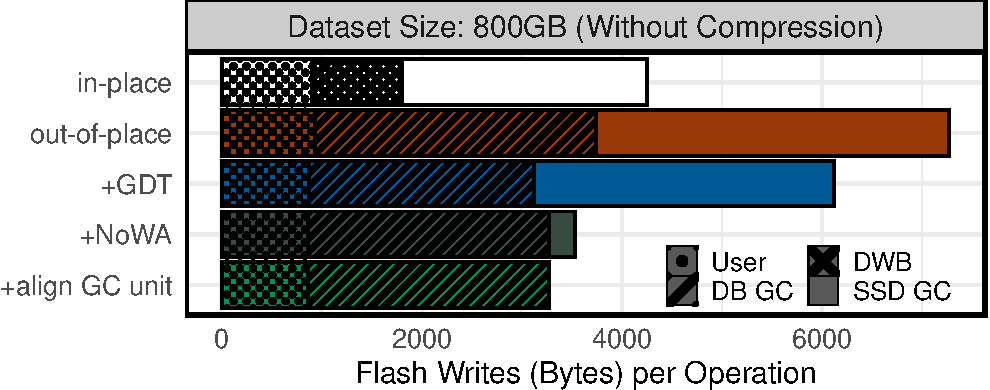
\includegraphics[width=\linewidth]{figures/writedrilldownohnecomp.pdf}
        \caption{Write drilldown without compression}
        \label{fig:drilldown:c}
    \end{subfigure}
    
    \caption{Total WAF on different dataset sizes and write drilldown with 800~GB dataset (YCSB-A zipf $\theta$ = 0.8, Samsung PM9A3)}
    \label{fig:drilldown}
\end{figure*}
%% TODO: add ssdiq benchmark zns-like workload
%% 8페이지반

